\chapter{Introducción}
El acceso seguro y fiable a la electricidad es clave para el desarrollo económico y social de
cualquier sociedad. Con el aumento de la demanda energética, se está acelerando la adopción
de energías renovables para combatir el cambio climático y reducir la dependencia de
combustibles fósiles\\%cite{quest2022indicator}.\\

La descarbonización del sistema energético y la mejora de la eficiencia en el uso de los
recursos presentan retos en la optimización de la producción, la gestión de la demanda y la
estabilidad de la red. Las infraestructuras deben adaptarse para integrar de forma eficiente
las energías renovables, sin aumentar los costes ni comprometer la calidad del suministro\\%\cite{khenissi2021pso}.\\

El consumo energético en los hogares ha evolucionado significativamente en los últimos años,
con un aumento en el uso de dispositivos electrónicos, electrodomésticos con mayor capacidad 
computacional y el auge del vehículo eléctrico (EV). Éste se ha convertido en una parte 
esencial de la transición hacia una movilidad más sostenible, pero su integración plantea 
desafíos significativos en términos de gestión de la demanda y estabilidad de la red 
eléctrica.\\

Los EV y vehículos híbridos enchufables (PHEV, por sus siglas en inglés) lejos están de ser 
tecnología del futuro, son el presente. Los EV y vehículos electrificados han cambiado por completo
el paradigma energético doméstico, convirtiéndose en una parte integral de la vida cotidiana%\cite{truong2021occupancy}.
La adopción de estos vehículos ha crecido exponencialmente en los últimos años, impulsada por
la necesidad de reducir las emisiones de gases de efecto invernadero y la dependencia de los
combustibles fósiles. En España, el número de vehículos eléctricos ha aumentado considerablemente,
con una creciente infraestructura de carga y un interés cada vez mayor por parte de los
consumidores.\\  

La carga de estos vehículos eléctricos puede generar picos de demanda que, de no ser
gestionados adecuadamente, podrían llegar a comprometer la fiabilidad de la red y aumentar 
significativamente los costes operativos~\cite{yao2005energy}, repercutiendo finalmente en los consumidores.
La \hyperref[fig:ev_interest]{\figurename~\ref*{fig:ev_interest}} muestra la evolución del 
interés por los EV en España durante los útlimos diez años\\

\begin{figure}[ht]
    \centering
    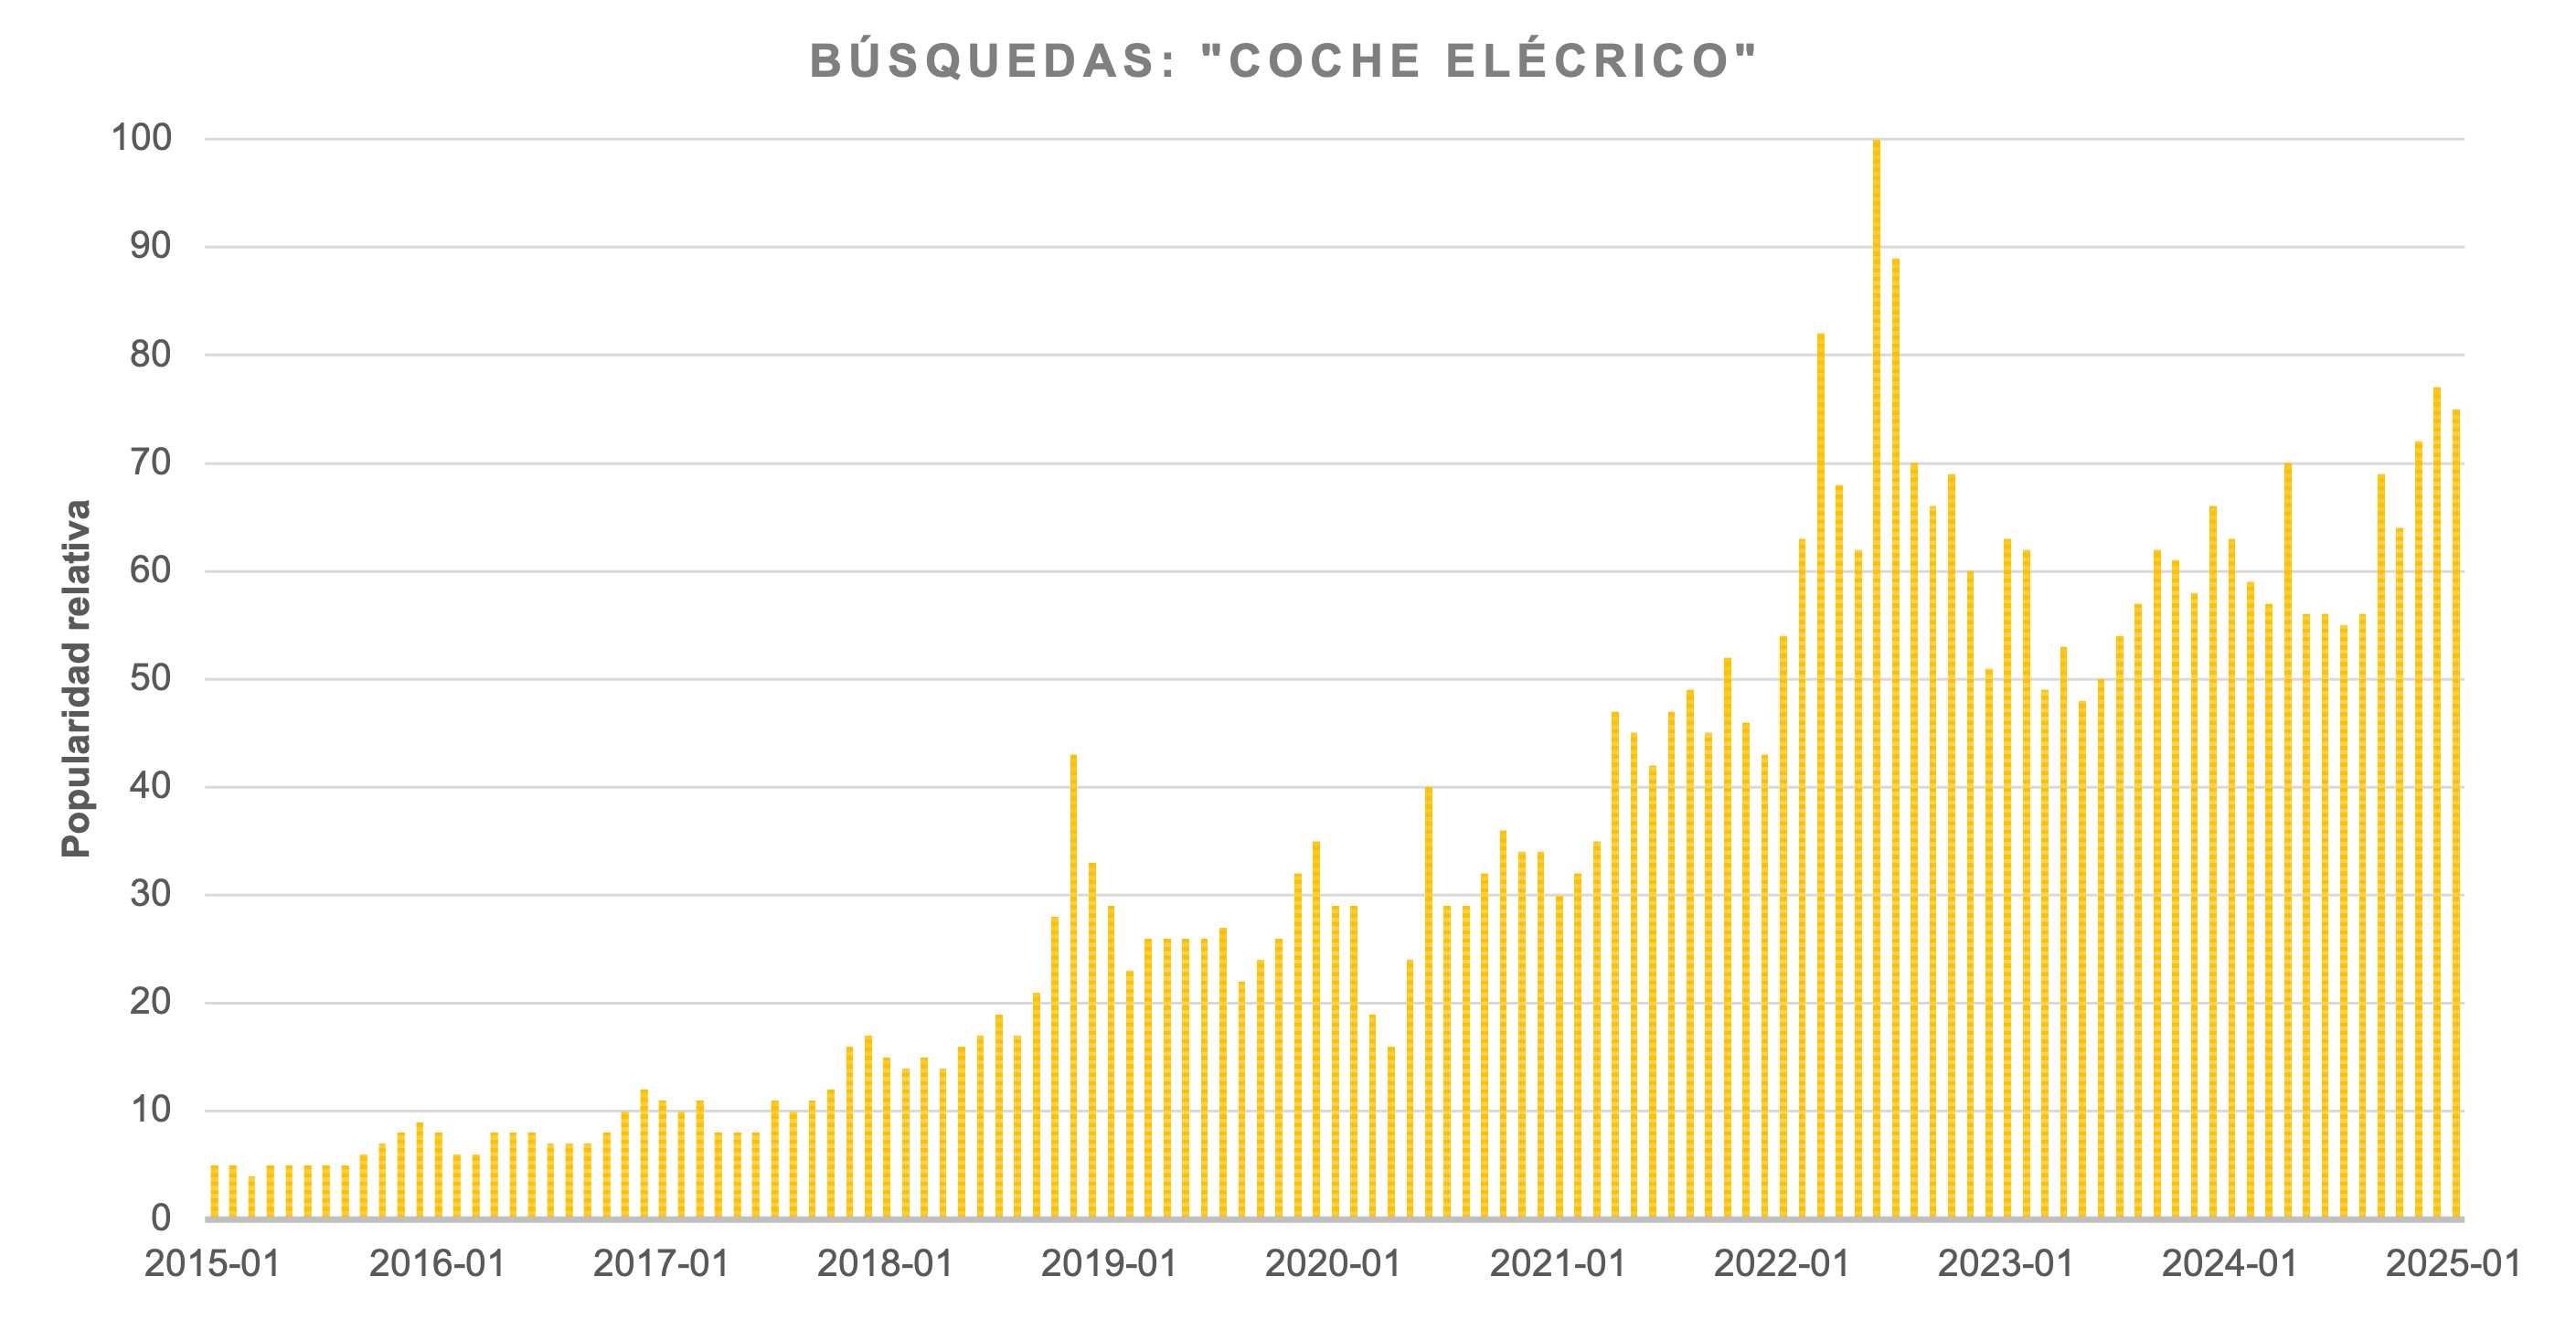
\includegraphics[width=1\textwidth]{images/EV_search_graph.png}
    \caption{Evolución del interés por los vehículos eléctricos en España (2015-2025). 
    Fuente: Google Trends~\cite{googletrends2025}}
    \label{fig:ev_interest}
\end{figure}

Además, la variabilidad en la disponibilidad de energía renovable, como la solar y la eólica,
las fuentes renovables más populares en nuestro país%\cite{kim2024renewable}
, introduce 
incertidumbre en la generación de energía. Esto, a su vez, requiere una gestión más dinámica 
y flexible de la demanda para garantizar un suministro estable y eficiente. La gestión de la 
carga de los vehículos eléctricos es un aspecto crítico para garantizar que la transición hacia 
un sistema de transporte sostenible no comprometa la estabilidad de la red eléctrica.\\

La Inteligencia Artificial Generativa (IA Generativa) surge como una herramienta
prometedora para enfrentar estos desafíos. Gracias a su capacidad de analizar grandes
volúmenes de datos en tiempo real, la IA Generativa puede predecir patrones de consumo,
optimizar la generación y distribución de energía, anticipar fallos en infraestructuras y
ajustar el consumo a las condiciones de la red de manera más eficiente y eficaz que los métodos
tradicionales.\\

La IA Generativa permite la creación de modelos predictivos que pueden simular diferentes
perfiles de carga, facilitando la toma de decisiones informadas y la implementación de estrategias
de gestión de la demanda más efectivas. Además, su capacidad para aprender y adaptarse a nuevas 
condiciones y entornos, la convierte en una herramienta valiosa para la planificación y operación 
de sistemas energéticos cada vez más complejos.

\section{Motivación}
La gestión responsable y eficiente de la energía es una tarea de vital importancia para una 
sociedad cada día más consciente y proactiva en tareas de sostenibilidad. Añadiendo a este panorama
el crecimiento experimentado por la movilidad eléctrica en el siglo XXI, dicha gestión eficiente y 
responsable del consumo energético aplica necesariamente a la carga de vehículos eléctricos.\\

La carga de estos vehículos puede generar picos de demanda que, si no se gestionan adecuadamente, 
pueden comprometer la fiabilidad de la red eléctrica y aumentar los costes operativos, 
repercutiendo finalmente en los consumidores. Además, la variabilidad en la disponibilidad de 
energía renovable, como la solar y la eólica, introduce incertidumbre en la generación de energía, 
lo que requiere una gestión más dinámica y flexible de la demanda para garantizar un suministro 
estable y eficiente.\\

Las innovadoras herramientas que presenta la IA Generativa, junto con las redes neuronales 
(Neural Networks, NN) basadas en aprendizaje por refuerzo (Reinforcement Learning, RL), exhiben 
un gran potencial para abordar estos retos de manera novedosa, y con resultados del más alto 
rendimiento.

\section{Objetivos}
El objetivo del proyecto es desarrollar in sistema gestor inteligente para la carga de EVs en un 
contexto dómestico. Para ello, se hará uso de técnicas de IA Generativa, RLNN (Reinforcement 
Learning Neural Network) y algoritmos clásicos de optimización.\\

El gestor deberá decidir, en base a una serie de restricciones y requisitos, tanto físicos como 
lógicos, si cargar o no el EV en un momento dado. Idealmente, el gestor conseguirá cargar el EV 
de la forma más eficiente posible, minimizando el coste de la carga y maximizando el uso de energía
disponible, al tiempo que se cumplen las restricciones impuestas por el usuario y las 
características del sistema eléctrico.\\

Para lograr este objetivo, se han definido unos objetivos secundarios específicos. El primero tiene
que ver con toda la parte generativa del proyecto: la creación de perfiles sintéticos de demanda no
gestionable, disponibilidad y requisitos del EV. En segundo lugar,se realizará una optimización 
clásica, tratando el problema de la carga como un pograma lineal (Linear Programme, LP), y se 
resolverá como tal. Con esta optimización clásica, que garantiza un resultado óptimo según las 
restricciones que se le impongan en forma de ecuación, se compararán los resultados de ambos 
métodos.\\

Se evaluarán tres métricas principales: coste incurrido en la carga, cuantía de energía empleada y 
rendimiento computacional.

\section{Estructura}
El trabajo está estructurado en seis capítulos, incluyendo este introductorio. Tras esta breve 
introducción, exposición de la motivación para el proyecto y los objetivos que se pretenden 
alcanzar, el segundo capítulo se centra en la revisión del estado del arte, donde se analizarán las 
técnicas de IA Generativa, las redes neuronales con aprendizaje por refuerzo y su aplicación en la 
gestión de la demanda energética.\\

El tercer capítulo presenta el diseño y desarrollo del sistema propuesto, incluyendo la 
arquitectura de la red neuronal y el enfoque de aprendizaje por refuerzo utilizado. Es decir, la 
metodología llevada a cabo durante el proyecto. El cuarto capítulo ofrece una explicación 
detallada de la implementación del sistema de acuerdo a lo explicado en el estado del arte, y 
contenido en el marco de la metodología. En este capítulo se detallan los algoritmos
implementados, las técnicas de IA Generativa utilizadas y la forma en que se integran para
lograr los objetivos del proyecto.\\

El quinto capítulo muestra una discusión de la comparación de los resultados obtenidos con los
diferentes enfoques - la optimización clásica y el sistema de RLNN + IAGen - y una evaluación 
de su rendimiento en términos de coste, eficiencia y rendimiento computacional. Finalmente, en
el sexto capítulo se presentan las conclusiones del proyecto, así como las posibles líneas de
investigación futura. Se reflexiona sobre los logros alcanzados, las lecciones aprendidas y
las implicaciones de los resultados obtenidos. Además, se discuten las posibles aplicaciones
prácticas del sistema desarrollado, dando fin al proyecto.\\ 

El trabajo se complementa con una serie de apéndices que incluyen detalles técnicos adicionales,
enlace al código fuente y otros materiales relevantes que respaldan la investigación y el 
desarrollo. Estos apéndices proporcionan una visión más profunda de los aspectos técnicos
del proyecto y permiten una comprensión más completa de los métodos y resultados presentados.

\vfill
